\subsection{External News-Corpus Validation: MultiHop-RAG}
\label{sec:mhrag_external}

MultiHop-RAG~\cite{tang2024multihoprag} supplies a news-document benchmark outside the Wikipedia-oriented tiers. The complete frozen release has 2,556 questions: retrieval and answer EM/F1 use 2,255 non-null questions; 301 null queries define separate canonical abstention. Support is matched by parent-document evidence IDs, rather than Wikipedia titles. Five available retrieval methods, two pinned readers and both 450/900-character evidence settings yield 20 sealed cells with 51,120 answers.

This is an available-condition analysis, not a complete six-condition transfer test. IRCoT is technically unavailable because the frozen local adapter assumes the HotpotQA corpus/index and lacks registered external parser, prompt, stopping and smoke anchors. This limits the implementation, not the IRCoT algorithm. Four observed contrasts versus BM25 use Holm correction with a fifth slot reserved conservatively at 1.0; no observed IRCoT $p$-value is imputed. The full registered family and transport decision are not complete.

% Generated by scripts/build_jiis_chatfix_tables.py; available evidence only.
\begin{table*}[!htbp]
\centering\footnotesize
\caption{MultiHop-RAG retrieval on 2,255 non-null queries (top-10).}
\label{tab:mhrag_retrieval}
\begin{threeparttable}
\setlength{\tabcolsep}{3pt}
\begin{tabular}{lrrrrlr}
\toprule
Method & Any & All & Recall & $\Delta$All & 95\% CI & $p_{\rm Holm}$ \\
\midrule
BM25 & 0.982 & 0.583 & 0.807 & -- & -- & -- \\
Dense BGE & 0.979 & 0.503 & 0.767 & -0.079 & [-0.098, -0.060] & $<0.001$ \\
Qwen-HyDE & 0.970 & 0.448 & 0.731 & -0.134 & [-0.155, -0.114] & $<0.001$ \\
Mistral-HyDE & 0.968 & 0.434 & 0.718 & -0.149 & [-0.169, -0.128] & $<0.001$ \\
Cross-encoder & 0.996 & 0.729 & 0.890 & +0.146 & [+0.127, +0.165] & $<0.001$ \\
\bottomrule
\end{tabular}
\begin{tablenotes}\scriptsize\item Parent-document evidence IDs define support; 301 null queries are excluded from retrieval denominators. Cross-encoder reranks a frozen BM25 top-100 pool. All-support and EM are primary endpoints. Four observed contrasts versus BM25 use Holm correction with a fifth slot conservatively reserved at 1.0 for unavailable IRCoT; this is not an observed IRCoT $p$-value. The full registered family is incomplete. Intervals are 95\% question-level bootstrap intervals (10,000 resamples); intervals alone do not determine significance.
\end{tablenotes}
\end{threeparttable}
\end{table*}


Complete-support retrieval is \MHRBMAll{} for BM25, \MHRDenseAll{} for Dense, \MHRQAll{} for Qwen-HyDE and \MHRMAll{} for Mistral-HyDE. All three adjusted contrasts with BM25 are negative. The cross-encoder reaches \MHRCEAll{}, with a positive adjusted gain of \MHRCEGain{} (Table~\ref{tab:mhrag_retrieval}). Standard open-generator expansion therefore supplies no observed gain over the lexical baseline here, while reranking the frozen BM25 top-100 pool does.

New post-hoc comparisons also match each expansion directly to the same Dense baseline on all 2,255 non-null IDs. All-support deltas are $-0.0550$ for Qwen-HyDE and $-0.0692$ for Mistral-HyDE, with Holm-adjusted $p=2.29\times10^{-11}$ and $3.24\times10^{-17}$. All eight reader/length EM comparisons favor Dense after adjustment. These additional families leave the historical BM25 family unchanged (Online Resource 1, Section~\SuppRef{sec:supp_priority_diagnostics}).

Retrieval improvement only partly carries through to answers. Cross-encoder EM gains over BM25 are positive after adjustment with both readers at 450 characters and Qwen at 900 characters; Mistral/900 remains unresolved. Both HyDE variants have negative adjusted EM contrasts with Qwen at both lengths; their Mistral contrasts are unresolved. Dense improves Mistral/900 EM, with the other EM contrasts unresolved. The exploratory EM interaction is significant only for Mistral-HyDE versus BM25 at 450 characters. Non-significant interactions do not establish reader invariance. Both lengths, secondary F1, raw/adapted scores and null abstention are retained in supplementary Section~\SuppRef{sec:supp_mhrag_external} in Online Resource 1.

Figure~\ref{fig:retrieval_answer_contrasts} summarizes the cross-encoder contrasts with BM25 across the three corpus-scale evaluations. Retrieval gains are supported in each, whereas the answer decisions depend on corpus, reader and, for news, character budget. The distinct support definitions and endpoints preclude a pooled gain or retrieval-to-answer conversion rate.

\begin{figure}[tbp]
\centering
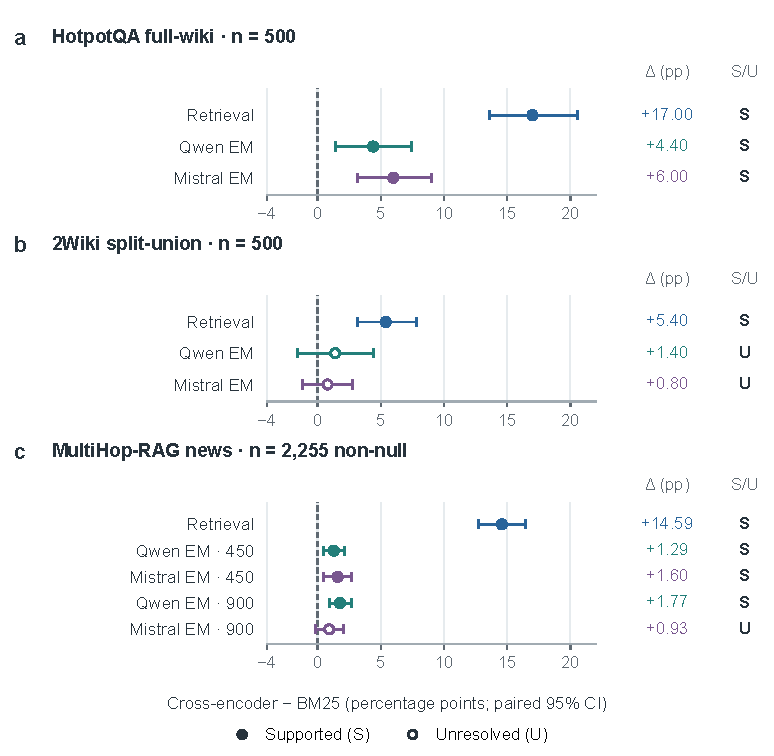
\includegraphics[width=\textwidth]{Fig3_RetrievalAnswer.pdf}
\caption{Retrieval and answer gains across evaluated configurations. Cross-encoder minus BM25 paired effects and reported 95\% bootstrap intervals on (a) HotpotQA full-wiki, (b) 2Wiki split-union and (c) MultiHop-RAG news. Retrieval is all-support hit@10; answer quality is exact match (EM). News labels 450/900 denote characters per document; retrieval is drawn once. Filled (S) and hollow (U) points preserve original Holm decisions. Wiki support uses titles; news support uses parent-document evidence IDs and excludes 301 null questions. Effects are not pooled across endpoints or corpora and do not estimate causal mediation.}
\label{fig:retrieval_answer_contrasts}
\end{figure}


Null queries expose a separate reader limitation. Mistral/900 canonical abstention is 0.0299 for both BM25 and the cross-encoder, compared with Qwen at 0.6611/0.6213. However, lexical refusal expressions occur in 170/301 and 153/301 Mistral outputs, respectively. This gap and frequent output-cap termination indicate a format-sensitive endpoint, rather than a human-confirmed hallucination rate. The registered adapter and canonical-null scores remain unchanged.

On the frozen 500-question prompt subset, query2doc-style improves all-support retrieval over standard for both generators after adjustment; evidence-only does not. Same-subset Dense and BM25 scores are 0.502 and 0.590, versus 0.516/0.512 for Qwen/Mistral Query2doc-style. The new 36-contrast post-hoc family leaves both Query2doc-versus-Dense comparisons unresolved and both contrasts with BM25 negative. Seed dispersion on the disjoint 300-question subset remains descriptive; alternative-prompt answer gains are unmeasured. Missing end-to-end costs prevent efficiency claims, and withdrawn independent human validation leaves evidence sufficiency unmeasured.
